\section{\system}
\label{sec:system}

{\system} is a visual authoring environment for constructing composite
visualizations from reusable chart blocks through layout-referenced
composition and data-aware adaptation.


\subsection{Design Rationale}
\label{sec:design-rationale}

Based on the design space, we derive two complementary design rationales for
{\system}. Both use visible visual structure as an authoring reference:
spatial layout provides a direct basis for reasoning about relationships among
blocks, while recognizable visual forms provide stable units for reasoning
about what should be composed.

\textbf{Layout as a Reference for Composition.}
Prior taxonomies~\cite{javed2012exploring,Composite,vaid} and our design space suggest that many
composition relationships are inherently expressed through spatial
organization. Layering, concatenation, and nesting correspond to recognizable
relative arrangements among visual units, making layout a natural reference
for composition. We therefore aim to make spatial relationships a primary
means for expressing and reasoning about composition intent, while keeping
intentional composition distinguishable from incidental arrangement.

\textbf{Visual Form as a Reference for Authoring.}
Our expert analysis further suggests that composite visualizations are often
perceived and decomposed at the level of recognizable chart forms rather than
fine-grained graphical elements. Established idioms such as stacked bars,
streamgraphs, and sunbursts carry distinct perceptual and semantic identities
even when they can be decomposed into simpler marks. We therefore aim to place
authoring reasoning at the level of meaningful visual units, allowing authors
to focus on selecting and relating recognizable forms rather than reconstructing
them from lower-level elements. At the same time, choosing such a unit should
not require an early commitment to the final data dimensional structure.



\subsection{Operationalizing the Design Space}

The preceding analysis defines the relationships that a block-based authoring
system should expose, but a prototype requires a concrete block vocabulary and
data format. We therefore instantiate the design space with a finite block
collection and a simplified data format.

\textbf{Block vocabulary and specifications.}
The block vocabulary was seeded from representative examples in D3~\cite{D3} and
deck.gl~\cite{deckgl}. Forms already covered by the expert-derived organization were assigned
to the corresponding families, while previously unseen forms were further
discussed with the experts to determine their block boundaries and family
memberships. The current prototype contains \textbf{45 unique chart blocks}
organized into \textbf{16 non-exclusive families}; a block may belong to
multiple families when it represents different perceptual alternatives.
For implementation, each block specifies its chart idiom, family memberships,
data requirements, encoding roles, dimensional capacity, spatial references,
and available structural targets. These specifications provide the information
needed for composition validation and dimensional adaptation. The complete
block inventory and block--family memberships are provided in the
supplementary material.

\textbf{Data format.}
The prototype uses a CSV-centered format for tabular, hierarchical, graph, and
geographic data. Tabular data requires no additional structural fields.
Hierarchical data requires node and parent identifiers to encode parent--child
relationships. Graph data requires node identifiers together with a separate
edge table whose source and target fields reference those nodes. Geographic
data uses a field in the tabular data to associate records with geometries
stored in an external GeoJSON file. These constraints provide a consistent
input format across the data structures supported by {\system}.

\subsection{Interface and Workflow}
\label{sec:interface}

The interface consists of four coordinated components: a Canvas, a Block List (Fig.~\ref{fig:BlockList}),
a Data Panel, and an Encoding Config Panel.

\textbf{Workflow.}
A typical authoring workflow begins with importing a dataset through the Data
Panel. {\system} automatically infers the semantic type of each column, after
which the author can inspect and correct the inferred types according to the
data semantics. To create an initial visualization, the author selects a chart
block from the Block List and drags it onto the Canvas. The chart can then be
configured either by dragging column names directly from the Data Panel to
available encoding channels or by assigning fields and adjusting visual
properties in the Encoding Config Panel. After configuring an individual
chart, the author can add further blocks and progressively compose them through
drag-and-drop operations. The resulting composition remains fully editable:
the author can revise its structure and composition-level properties, enter
individual chart blocks to modify their encodings, or update data assignments
without reconstructing the visualization.

\begin{figure}[ht]
\centering

\includegraphics[width=\columnwidth]{figs/polar_scale.pdf}
\caption{Coordinate-aware resizing of a polar block. Angular and radial
handles independently adjust its $\theta$ range and $r$ extent.}
\label{fig:polar-scale}

\end{figure}

\textbf{Canvas} supports arranging, composing, and editing chart blocks.
Authors can move, resize, and select blocks directly, with spatial manipulation
adapted to coordinate systems. Cartesian blocks are resized along $x$
and $y$, while polar blocks expose independent controls over angular
($\theta$) and radial ($r$) extents (Fig.~\ref{fig:polar-scale}). Dragging one
block relative to another invokes applicable composition targets, while an
existing composition can be manipulated as a unit or entered for internal
editing.








\begin{figure}[ht]
\centering
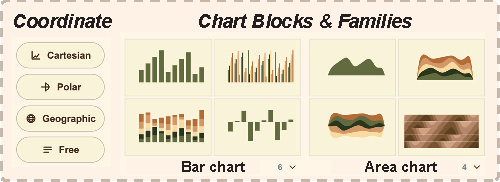
\includegraphics[width=\columnwidth]{figs/chartblocks.pdf}
\caption{Block List filters blocks by coordinate system and organizes
perceptually related alternatives into families.}
\label{fig:BlockList}

\end{figure}




\textbf{Block List} supports browsing and selecting chart blocks
(Fig.~\ref{fig:BlockList}). Blocks are organized by coordinate system and
perceptually related families, allowing authors to inspect related visual forms
and choose a block to place on the Canvas. A block may appear in multiple
families when it is relevant to different alternatives, while perceptually
distinct idioms remain separate choices.


\begin{figure}[ht]
\centering

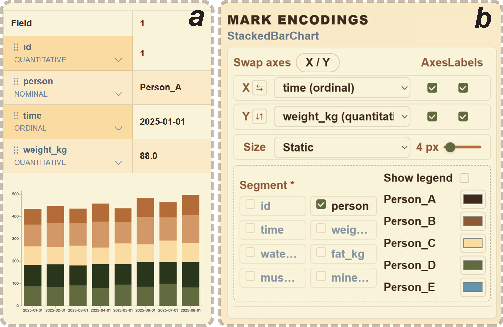
\includegraphics[width=\columnwidth]{figs/data-encoding.pdf}
\caption{Data and encoding configuration in {\system}: (a) field inspection
and assignment, and (b) block- and composition-level configuration.}
\label{fig:encoding}

\end{figure}



\begin{figure*}[t]
\centering

\includegraphics[width=\linewidth]{figs/interaction.pdf}

\caption{Drag-and-drop interactions for composing chart blocks.
(A) Dropping a block into another block's plotting region creates layering by
sharing both spatial dimensions.
(B) Dropping along a boundary creates concatenation; the boundary determines
the shared dimension and block order. The same interaction extends to polar
coordinates through angular and radial boundaries.
(C) Dropping onto an internal mark or structural element creates nesting,
replacing or overlaying repeated elements while inheriting their data and
spatial references.
}

\label{fig:interaction}

\end{figure*}

\begin{figure}[h]
\centering
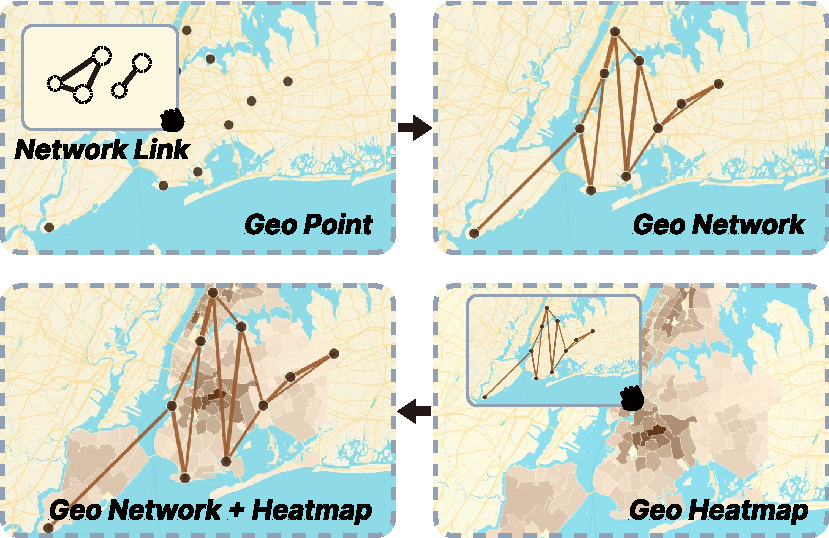
\includegraphics[width=\columnwidth]{figs/map_layer.pdf}
\caption{Layer composition in geographic visualization. Top: layering a
network-link block over geographic points forms a geographic network, with
links derived from the node positions. Bottom: the resulting network is
further layered with a geographic heatmap, combining network structure and
spatial density within the same geographic reference.}
\label{fig:geo-layer}

\end{figure}

\textbf{Data Panel} supports importing data, inspecting field information, and
assigning fields to chart blocks (Fig.~\ref{fig:encoding}.a). Most supported
data types use a single CSV file, while network data uses separate node and
link CSV files. The panel displays the inferred semantic type of each field and
allows authors to correct it when needed. Fields can be assigned either by
dragging them to specific encoding channels in the Encoding Config Panel or,
when the desired channel is unspecified, by dropping them directly onto a
chart, in which case {\system} presents applicable assignments or adaptation
options.



\textbf{Encoding Config Panel} supports binding data columns to available
encoding channels and configuring the corresponding visual encodings
(Fig.~\ref{fig:encoding}.b). For an individual block, authors can inspect and
modify field assignments, scales, and appearance properties. A composition can
be configured in the same panel: in addition to relationship properties such
as ordering, spacing, and alignment, authors can bind fields to
composition-level axes or other structural encodings. The panel also reports
incompatible assignments and available adaptation options.















\subsection{Direct Manipulation for Composition}

{\system} uses spatial drop semantics to construct compositions. During a drag,
it displays valid drop regions. Authors commits the composition by releasing the
dragged block over a region.

\subsubsection{Spatial Drop Semantics}



The position of a drop determines the composition operator
(Fig.~\ref{fig:interaction}). Interior drops create layers, boundary drops create
concatenations, and drops on internal structural targets create nested
compositions.



\textbf{Layering through interior drops.}
Dropping a chart block on the interior of another chart creates a layer
composition (Fig.~\ref{fig:interaction}.A). The blocks share a visual region
while retaining their own data assignments and encodings. Layering is
particularly common in geographic visualization, where multiple data layers
can be overlaid within a shared geographic reference, as in systems such as
deck.gl~\cite{deckgl}.
{\system} also represents networks through composable node and link layers.
A node layer can be any compatible point-based block, while a network-link
block derives its endpoints from the referenced nodes. Layering a link block
over geographic points therefore forms a geographic network, which can itself
be combined with additional geographic layers such as a heatmap
(Fig.~\ref{fig:geo-layer}). The constituent layers remain independently
editable while sharing the same geographic reference.




\textbf{Concatenation through boundary drops.}
Dropping a chart block near a boundary of the target creates a concatenation
(Fig.~\ref{fig:interaction}.B). For Cartesian charts, dropping near the left or
right boundary creates a horizontal concatenation, whereas dropping near the
top or bottom boundary creates a vertical concatenation.
For polar charts, {\system} defines four boundary drop areas corresponding to
two concatenation structures: \emph{angular concatenation} and \emph{radial
concatenation}. Drop areas for angular concatenation lie along the two
radial boundaries of the polar chart. Dropping a block on either boundary
places the two charts in adjacent angular sectors while preserving a shared
radial scale. Drop areas for radial concatenation lie along
the inner and outer circular boundaries. Dropping on either circular boundary
places the charts in concentric radial bands while preserving a shared angular
scale.


\textbf{Nesting through structural-target drops.}
Nesting associates a child chart with a repeated class of elements in a parent
chart (Fig.~\ref{fig:interaction}.C). During dragging, the author can
progressively enter the target's internal structure and drop the block at the
intended structural level. {\system} then creates one child instance for each
eligible parent element and establishes the corresponding data context.
Although the child may be rendered multiple times, it remains a single
configurable chart block. The progressive target-selection mechanism is
described in Sec.~\ref{sec:progressive-target-selection}.

\subsubsection{Progressive Target Selection}
\label{sec:progressive-target-selection}



A pointer location may correspond to multiple structural levels. In a stacked
bar chart, for example, a dragged block may target the complete chart, a bar,
or a segment, leading respectively to chart-level composition or nesting at
different internal levels.

\begin{figure}[ht]
\centering
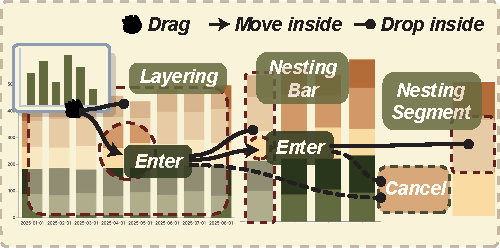
\includegraphics[width=\columnwidth]{figs/enter.pdf}
\caption{Progressive target selection across structural levels. Before entering
the target, dropping on the chart triggers layering. Entering the stacked-bar
structure exposes bars as nesting targets, and entering a bar further exposes
its segments. Dropping at these levels creates bar-level and segment-level
nesting, respectively.}
\label{fig:enter}

\end{figure}


{\system} resolves this ambiguity through progressive target selection
(Fig.~\ref{fig:enter}). A drag first exposes targets for the complete block and
an \emph{enter region} for accessing its internal structure. Entering this
region advances to the next level without committing an operation and updates
the available targets. Authors can continue until the intended structural
level becomes active.
At each level, {\system} highlights the active structural class and previews
the resulting instances. A drop applies to the corresponding class rather than
only the rendered element under the pointer, so nesting on one segment, for
example, applies to all eligible segments generated by that structure. The same
mechanism extends through existing compositions, while moving into empty canvas
space cancels the active target and returns to free dragging.



\subsubsection{Editing Compositions}
\label{sec:editing-compositions}

After a composition is created, {\system} preserves it as an explicit and
editable structure. Authors can configure the composition itself or enter it
to refine its constituent blocks.

\textbf{Configuring composition relationships.}
Selecting a composition exposes properties specific to its composition type.
Layering supports layer ordering and shared scales, concatenation controls
alignment and spacing, and faceting allows fields to be bound to facet axes.
For nesting, child blocks are initially centered on their parent elements, but
authors can refine their placement in Position Config Panel using
nine-point parent--child anchors and relative offsets
(Fig.~\ref{fig:compose}.a). Parent elements can be retained or hidden, and
optional borders can be added to child blocks to further adjust their visual
separation.

\begin{figure}[ht]
\centering

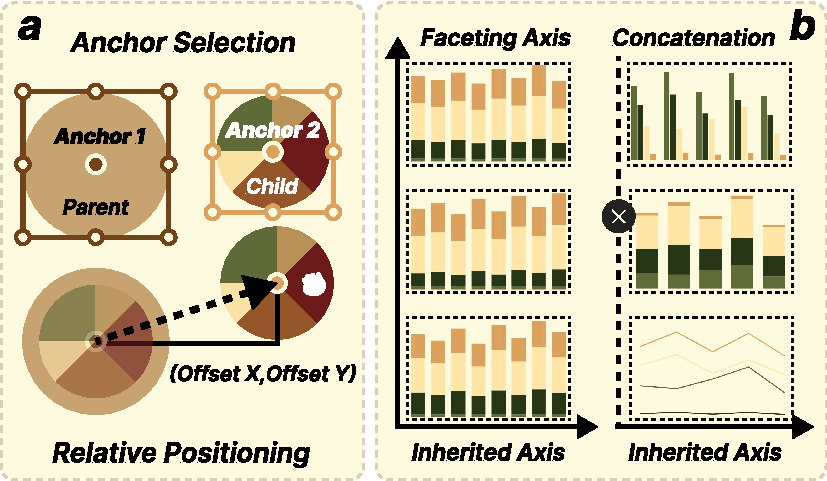
\includegraphics[width=\columnwidth]{figs/compose.pdf}
\caption{Configuration and spatial references of composed structures.
(a) Nested children can be repositioned using parent--child anchors and an
$(x,y)$ offset. (b) Faceting introduces a facet axis while inheriting the
remaining axis from its constituent block; concatenation inherits existing
axes without introducing a new coordinate dimension.}
\label{fig:compose}

\end{figure}


\textbf{Recomposing composite units.}
A composition is treated as a new authoring unit whose exposed axes and
repeated structures determine how it can participate in subsequent
composition. Faceting introduces a new facet axis
while inheriting the remaining axis from its constituent block, whereas
concatenation introduces no new axis and only inherits compatible axes from
its constituents(Fig.~\ref{fig:compose}.b). Repeated groups produced by faceting or nesting can further
serve as nesting targets. A layered or concatenated composition can also be
faceted when its constituent blocks share a compatible partitioning
dimension. Subsequent composition therefore operates on the axes and repeated
structures exposed by the composite unit while preserving its internal
relationships.









% \subsection{Data Compatibility and Adaptation}
% \label{sec:compatibility}

% {\system} reduces authors' need to anticipate data dimensionality while
% preserving meaningful relationships among chart blocks. The following sections
% describe the data semantics and chart contracts underlying this approach,
% followed by aggregation, adaptation across related blocks, and inherited data
% contexts in nested compositions.

% \subsubsection{Data Semantics and Chart Contracts}
% \label{sec:chart-contracts}

% Following the multidimensional data model underlying data cubes
% ~\cite{datacube}, {\system} treats the distinction
% between dimensions and measures as the primary analytical semantics of a data
% field. Dimensions organize observations according to attributes of interest,
% whereas measures represent the values examined with respect to those
% dimensions. Because this distinction describes how a field participates in an
% analysis, it forms the basis of the data model exposed to authors.

% To minimize the concepts authors must specify, {\system} only introduces
% additional distinctions when they directly affect the interpretation of a
% field. Dimensions are further classified as nominal or ordinal. Nominal
% dimensions identify unordered categories, whereas ordinal dimensions establish
% a meaningful order among their values. Measures are not exposed through a
% corresponding set of semantic subtypes because primitive types do not
% necessarily determine how a field should be interpreted. For example, two
% quantitative measures may still be incompatible because they have different
% units, ranges, or analytical meanings. Similarly, a temporal field may function
% as an ordinal dimension when it orders observations in a time series, or as a
% measure when it records the time associated with an individual observation.
% {\system} therefore handles primitive numeric and temporal types internally for
% parsing and scale construction rather than exposing them as additional
% semantics, which would increase authors' specification burden without
% clarifying a field's analytical role or compatibility.

% Each chart block defines a \textbf{contract} over this data model. The contract
% specifies its required channels, the analytical roles and ordering properties
% accepted by those channels, and the number of dimensions and measures that the
% block can represent. {\system} uses this contract to distinguish a semantically
% invalid assignment from a valid assignment that exceeds the current block's
% representational capacity. 

% In addition to the analytical roles accepted by its channels, the contract specifies a
% minimal set of channels required to instantiate the block and a maximal set
% that the block can represent. The former ensures that the block has sufficient
% data to produce a meaningful visualization, while the latter defines its
% representational capacity.

% To further determine whether an assigned dataset has the granularity required by a
% block's visual structure, each chart contract specifies a uniqueness
% constraint. Drawing on the data-cube model, we treat the fields assigned to
% visual channels as dimensions that jointly identify a cube state, and use the
% constraint to characterize the granularity expected by the block. We denote
% this constraint as $\mathit{unique}(c_1, c_2, \ldots, c_k)$, meaning that each
% combination of values assigned to channels $c_1, c_2, \ldots, c_k$ must
% correspond to at most one visual data item. For example, a single-line block
% requires $\mathit{unique}(x)$ because each position on its horizontal axis can
% be associated with at most one value on the line. This constraint allows
% {\system} to determine whether the assigned data already forms a valid
% state required by blocks.

% \subsubsection{Flexible Dimensionality through Aggregation}
% \label{sec:data-semantics}

% To improve compatibility between data and chart blocks, {\system} adopts the
% aggregation model introduced by data cubes, which allows the system to derive
% the data granularity required by a block rather than requiring the input data
% to match that granularity in advance.

% Aggregation is guided by the uniqueness constraints in contract.
% After fields are assigned to channels, {\system} examines whether the resulting
% data satisfies the specified constraint. If multiple records share the same
% combination of values on these channels, the system groups those records by
% the required channel values and aggregates their measures until each
% combination corresponds to a unique visual data item.
% For example, if $x$ represents year and $color$ represents region,
% $\mathit{unique}(x, color)$ requires one measure value for each year--region
% combination. If multiple records belong to the same combination, their
% measures are aggregated to produce a unique visual data item. Authors may
% override the default aggregation function when it does not reflect their
% analytical intent.


% By deriving aggregation from block contracts, {\system} separates the
% granularity of the raw data from the granularity required by a visualization.
% A block can therefore remain applicable across datasets with different record
% structures, while its contract ensures that the resulting data has a unique
% and valid visual interpretation.

% \subsubsection{Faceting and Family-level Adaptation}
% \label{sec:compositional-adaptation}

% A consequence of block-based authoring is that each block accepts only the
% data dimensions defined by its contract. This explicit capacity makes
% blocks predictable and reusable, but it can also prevent an additional
% dimension from being represented within the current block. 


% Faceting provides a general way to accommodate an additional dimension by
% partitioning the data. However, an author may not intend to create a faceted
% design; the selected block may simply lack the capacity to represent the
% dimension. In such cases, transitioning to a related block allows the dimension
% to be incorporated into a shared visual structure while preserving the
% author's existing design choices where possible.
% To provide such alternatives, {\system} connects blocks with
% different data capacities within the same chart family. For example, a
% single-line chart can transition to a multi-line chart, while a single-bar
% chart can transition to a grouped or stacked bar chart. The system transfers
% compatible field assignments, aggregation choices, and appearance properties
% to each applicable block, while the target block introduces the channels or
% structures needed to represent the additional dimension.


% \subsubsection{Data Context in Nested Compositions}
% \label{sec:nested-data-context}

% The configuration panel allows authors to precisely control how filters are
% inherited between a parent and its nested children. However, requiring such
% relationships to be configured before trying would impose
% substantial dimensional reasoning overhead. Following our principle that
% design exploration should support low-cost trial and error, {\system} provides
% a position-derived data context as the default, while retaining explicit
% configuration for authors with more precise intentions.

% Following the data-cube model, each nestable element corresponds to a partial
% coordinate defined by the dimension values represented at that structural
% level. By default, placing a child at an element fixes these values and passes
% them to the child as inherited filters. Authors therefore only need to assign
% the child's own channels to try the composition; its grouping and aggregation
% are evaluated over the records selected by the nesting position.
% For example, consider a stacked bar chart in which bars represent years and
% segments represent regions. A child placed at the bar level inherits the
% corresponding year, producing one instance for each year. A child placed at the
% segment level inherits both year and region, producing one instance for each
% year--region combination. All instances share the same child block and channel
% assignments, while their data contexts are determined by their respective
% positions. Authors can subsequently refine this default behavior in the
% configuration panel by modifying or disabling the inherited filters.

\subsection{Dimensional Continuity and Adaptation}
\label{sec:compatibility}

Under block-based authoring, each block provides an explicit visual form with
bounded dimensional capacity. After completing the block's required
assignments, authors can introduce an additional field by dropping its column
onto the chart. If the field is semantically compatible but exceeds the
block's capacity, {\system} treats the assignment as an adaptation point,
allowing the added dimension to be accommodated without reconstructing the
design.



\textbf{Chart-level data capacity.}
Following the multidimensional model of data cubes~\cite{datacube}, {\system}
uses dimensions and measures as the primary analytical roles of data fields.
Each block defines a contract specifying its accepted encoding roles, minimum
assignments, and dimensional capacity. Blocks that summarize records may also
define a uniqueness constraint,
$\mathit{unique}(c_1,c_2,\ldots,c_k)$, requiring each combination of channel
values to correspond to at most one visual item; {\system} aggregates records
when necessary to satisfy this constraint. Record-preserving blocks, such as
scatterplots, trees, and networks, do not require such aggregation.

\textbf{Adaptation at form boundaries.}
When an additional dimension exceeds the capacity of the current block,
{\system} exposes two alternatives. The dimension can be absorbed into a
related family member with greater capacity, such as transitioning from a
single-line to a multi-line block or from a basic bar to a grouped or stacked
variant. Alternatively, the current block can be retained and the dimension
externalized through faceting. Compatible field assignments, aggregation
choices, and appearance properties are preserved across these adaptations.
The two alternatives therefore expose different structural consequences of
the same dimensional extension: changing the internal visual form or
introducing structure at the composition level.

\textbf{Position-derived nesting context.}
Authors can retain the current block and place it within an existing structure.
{\system} automatically derives the child's data context from its nesting
level and position: each nested instance inherits the dimension values
represented by the corresponding parent element as filters. This allows the
block to operate under different dimensional contexts without changing its
visual form.

